
% Resume in Latex
% Author : Diego Renner
% Based on: Sourabh Bajaj repo
% License : MIT
%------------------------

\documentclass[letterpaper,11pt]{article}

\usepackage{latexsym}
\usepackage[empty]{fullpage}
\usepackage{titlesec}
\usepackage{marvosym}
\usepackage[usenames,dvipsnames]{color}
\usepackage{verbatim}
\usepackage{enumitem}
\usepackage[hidelinks]{hyperref}
\usepackage{fancyhdr}
\usepackage[english]{babel}
\usepackage{tabularx}
\usepackage{lmodern}
\usepackage{anyfontsize}
\usepackage[export]{adjustbox}
\usepackage{wrapfig}
\usepackage{graphicx}

% Page coloring, fonts, and logos
\usepackage{pagecolor}
\usepackage{lato}
\renewcommand{\familydefault}{\sfdefault}
\usepackage{fontawesome}
% ---

\pagestyle{plain}
\fancyhf{} % clear all header and footer fields
\fancyfoot{}
\renewcommand{\headrulewidth}{0pt}
\renewcommand{\footrulewidth}{0pt}

% Adjust margins
\addtolength{\oddsidemargin}{-0.5in}
\addtolength{\evensidemargin}{-0.5in}
\addtolength{\textwidth}{1in}
\addtolength{\topmargin}{-.5in}
\addtolength{\textheight}{1.0in}
\urlstyle{same}
\raggedbottom
\raggedright
\setlength{\tabcolsep}{0in}
% ---

% Sections formatting
\titleformat{\section}{
	\vspace{-4pt}\scshape\raggedright\large }{}{0em}{}[\color{black}\titlerule \vspace{-5pt}]
% ---

% Custom commands
\newcommand{\resumeItem}[1]{%2
\item\small{
		%\textbf{#1}
		#1
		%{: #2 \vspace{-2pt}}
	}
}

\newcommand{\resumeSubheading}[4]{
	\vspace{8pt}\item%-1
	\begin{tabular*}{0.97\textwidth}[t]{l@{\extracolsep{\fill}}r}
		\textbf{#1} & #2 \\
		\textit{\small#3} & \textit{\small #4} \\
	\end{tabular*}\vspace{-5pt}
}
\newcommand{\resumeSubSubheading}[2]{
	\vspace{1pt}
	\begin{tabular*}{0.97\textwidth}{l@{\extracolsep{\fill}}r}
		\textit{\small#1} & \textit{\small #2} \\
	\end{tabular*}\vspace{-5pt}
}
\newcommand{\resumeSubItem}[2]{\resumeItem{#1}{#2}\vspace{-4pt}}
\renewcommand{\labelitemii}{$\circ$}
\newcommand{\resumeSubHeadingListStart}{\begin{itemize}[leftmargin=*]}
\newcommand{\resumeSubHeadingListEnd}{\end{itemize}}
\newcommand{\resumeItemListStart}{\begin{itemize}}
\newcommand{\resumeItemListEnd}{\end{itemize}\vspace{-5pt}}

\newcommand{\resumeTech}[2]{
	\textbf{#1:} #2
}

% COLOR THEMES SELECTION
% For Light theme un-comment this and comment the Dark theme section below
% \colorlet{urlcolor}{blue}
% \newcommand{\otherThemeRef}{\href{https://github.com/DiegoRenner/CV/blob/master/CV_dark.pdf}{See dark theme}}
% \newcommand{\latestVersion}{\href{https://github.com/DiegoRenner/CV/blob/master/CV_light.pdf}{Get Latest version}}

\input{\jobname.theme}
% For Dark theme un-comment this and comment the Light theme section above

%\colorlet{textcolor}{white!80!gray}
%\colorlet{backgroundcolor}{black!30!gray}
%\colorlet{urlcolor}{blue!25!white}
%\AtBeginDocument{\color{textcolor}}
%\newcommand{\otherThemeRef}{\href{https://github.com/DiegoRenner/CV/blob/master/CV_light.pdf}{See light theme}}
%\newcommand{\latestVersion}{\href{https://github.com/DiegoRenner/CV/blob/master/CV_dark.pdf}{Get Latest version}}
% ---

% DOCUMENT MAIN
\begin{document}


% HEADING
%\begin{tabular*}{\textwidth}{l@{\extracolsep{\fill}}r}
%	\textbf{\href{https://www.linkedin.com/in/diego-renner-6169851b5/}{\Large Diego Renner}} &  \href{https://github.com/DiegoRenner}{ \faicon{github} \color{urlcolor} DiegoRenner} \\
%	\href{mailto:diego.renner@sam.math.ethz.ch}{diego.renner@sam.math.ethz.ch} &  \faicon{code} C++, Python, Java\\
%	\textsl{\small \latestVersion} & \textsl{\small \otherThemeRef}
%\end{tabular*}
%\begin{wrapfigure}{R}{10cm}
%	\centering
%	\includegraphics[10cm]{diego-23.jpg}
%\end{wrapfigure}
\begin{minipage}[T]{0.3\textwidth}
\begin{tabular*}{\textwidth}{l}

	\textbf{\href{https://www.linkedin.com/in/diego-renner-6169851b5/}{\Large Diego Renner}} \\
	\href{mailto:diego@plantime.io}{diego@plantime.io}\\
	\href{tel:+41763948608}{+41 76 394 86 08} \\
	\\
	\href{https://github.com/DiegoRenner}{ \faicon{github} \color{urlcolor} DiegoRenner} \\
	\faicon{code} \href{https://github.com/DiegoRenner/HelmholtzTransmissionProblemBEM}{C++}, \href{https://github.com/DiegoRenner/jaxFlowSim}{Python}, \href{https://www.plantime.io/}{Rust}\\
	\\
	Date of Birth: 29.08.1995 \\
	Nationality: Swiss \\
	\\
	\textsl{\small \latestVersion} \\
	\textsl{\small \otherThemeRef} \\
	\hfill \textsl{(Items relating to projects and papers are clickable.)}



\end{tabular*}
\end{minipage}
\begin{minipage}[T]{0.69\textwidth}
		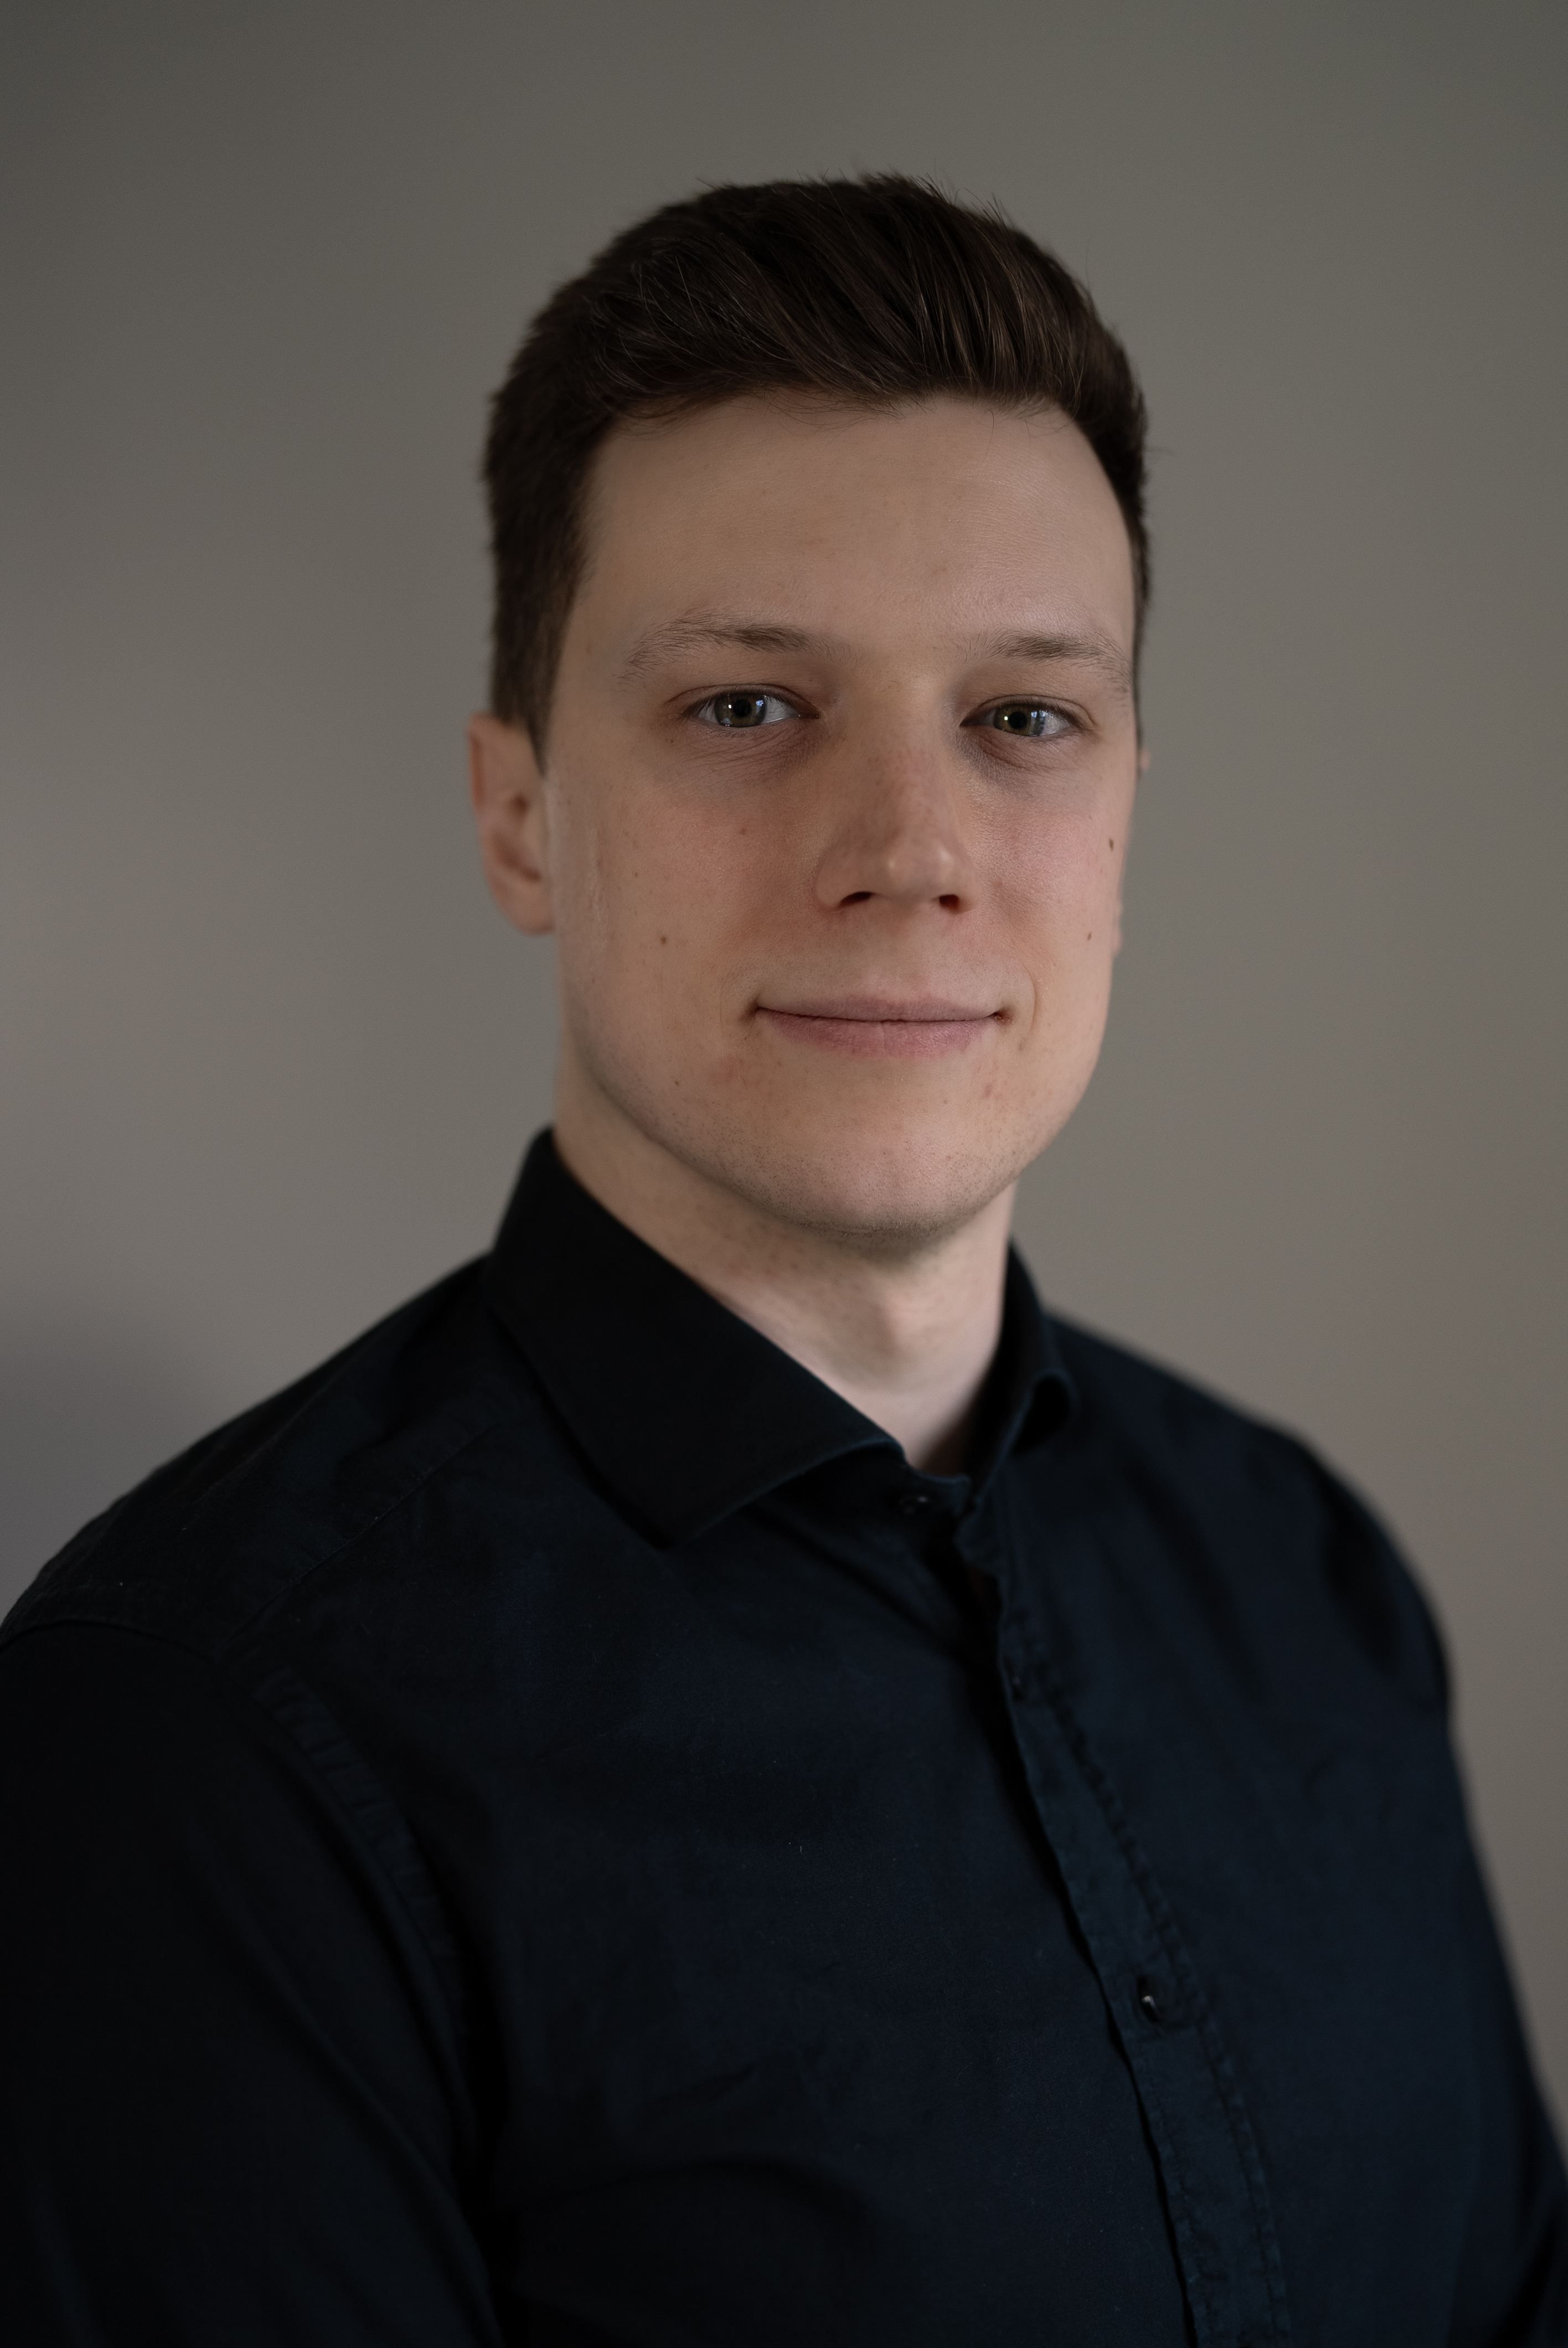
\includegraphics[width=0.5\textwidth, right]{portrait.jpg}
\end{minipage}
% ---

% EDUCATION
\section{Education}
\resumeSubHeadingListStart
\resumeSubheading
{ETH Zurich}{Zurich, Switzerland}
{M.Sc. Mathematics}{September 2021 - December 2023}
\resumeItemListStart
\resumeItem{\href{https://github.com/DiegoRenner/jaxFlowSim}{Degree completed with a thesis on differentiable haemodynamics solver in JAX (Python).}}
\resumeItemListEnd
\resumeSubheading
{ETH Zurich}{Zurich, Switzerland}
{M.Sc. Computational Science and Engineering, Specialization Physics}{September 2018 - August 2021}
\resumeItemListStart
\resumeItem{\href{https://github.com/DiegoRenner/HelmholtzTransmissionProblemBEM}{Degree completed with a thesis on solving the transmission scattering problem using BEM (C++).}}
\resumeItemListEnd
\resumeSubheading
{University of Basel}{Basel, Switzerland}
{B.Sc. Computational Mathematics}{September 2014 - December 2017}
\resumeItemListStart
\resumeItem{Completed extracurricular courses on Computer Architecture, Operating Systems and Quantum Mechanics.}
\resumeItemListEnd
\resumeSubheading
{Gymnasium Bäumlihof}{Basel, Switzerland}
{Matura, Specialization Biology \& Chemistry}{August 2009 - July 2014}
\resumeSubHeadingListEnd
% ---

% PROJECTS
\section{Projects \& Thesis}

\resumeSubHeadingListStart
\resumeSubItem{\href{https://github.com/ktrianta/n-body-problem}{Parallelizing the Barnes-Hut Algorithm with MPI: Parallelized implementation of N-Body solver in C++ using the MPI framework. (Course Work)}}

\resumeSubItem{\href{https://github.com/DiegoRenner/phonons}{AiiDA Lab implementation of IR spectrum calculations for carbon based nanomaterials: An AiiDa workflow implemented in the Jupyter Notebooks based AiiDa lab interface. (Semesters Thesis, Computational Science)}}

\resumeSubItem{\href{https://github.com/DiegoRenner/HelmholtzTransmissionProblemBEM}{Near Resonances for Scattering Transmission Problems: A BEM based C++ solver for Scattering Transmission Problems, developed to investigate scatterer-dependent near resonances. (Master's Thesis, Computational Science)}}


\resumeSubItem{\href{https://github.com/DiegoRenner/Game-Sim-ML-in-Finances-}{ML Based Game Simulation in a Finance Setting: Agents trained to trade or hold a stock taking into account real historical data on cash returns. Policies are learned via reinforcement learning. (Course Work)}}

\resumeSubItem{\href{https://github.com/camlab-ethz/jaxFlowSim}{On differentiable simulations of haemodynamic systems: A 1D-haemodynamics solver written in Python using JAX. The differentiability of the solver aims to aid in the development of personalised medicine. (Master's Thesis, Mathematics)}}

\resumeSubHeadingListEnd
% ---

% PROJECTS
\section{Publications}

\resumeSubHeadingListStart
\resumeSubItem{\href{https://www.researchgate.net/publication/372765555_Detecting_Near_Resonances_in_Acoustic_Scattering}{Detecting Near Resonances in Acoustic Scattering: Continued development of root finding algorithm from Master's Thesis using handcrafted optimization algorithm and state of the art computation of singular values. (Published)}}

\resumeSubItem{\href{https://arxiv.org/abs/2412.14572}{Accelerated Patient-Specific Calibration via Differentiable Haemodynamics Simulations: Demonstrating feasibility of parameter inference through differentiable 1D-haemodynamics solver written in Master's Thesis. (Preprint)}}

\resumeSubItem{Raman spectroscopy enabled automatic media release controlled by convolutional neural networks. (Work in Progress)}{}
\resumeSubHeadingListEnd
% ---

% EXPERIENCE
\section{Experience}
\resumeSubHeadingListStart


\resumeSubheading
{Novartis Pharma AG}{Basel, Switzerland}
{MSc Student Proc Dev \& New Technologies}{June 2024 - December 2024}
\resumeItemListStart
\resumeItem{Developing ML/AI algorithms for classifying Raman spectroscopy data.}
\resumeItemListEnd
\resumeTech{Technologies}{imbalanced-learn, JAX, Matplotlib, NumPy, scikit-learn, SciPy, TensorFlow}\\
\resumeTech{Theory}{(C)NN, DoE, GMM, PCA, SMOTE}

\resumeSubheading
{\href{https://www.plantime.io/}{plantime}}{Basel, Switzerland}
{Software Engineer}{January 2024 - May 2024}
\resumeItemListStart
\resumeItem{Developing ML/AI algorithms for optimizing shift scheduling.}
\resumeItemListEnd
\resumeTech{Technologies}{Rust}\\
\resumeTech{Theory}{Evolutionary optimization algorithms}

\resumeSubheading
{ETH Zurich}{Zurich, Switzerland}
{Teaching Assistant}{September 2021 - February 2022}
\resumeItemListStart
\resumeItem{Teaching Assistant for Lecture "Numerical Methods for Computer Science".}
\resumeItemListEnd
\resumeTech{Technologies}{C++}\\
\resumeTech{Theory}{ODEs, PDEs and numerical algorithms to solve them}

\resumeSubheading
{ETH Zurich}{Zurich, Switzerland}
{Research Assistant}{September 2020 - June 2021}
\resumeItemListStart
\resumeItem{Hired for continued development of BEM code that was implemented in Master's Thesis.}
\resumeItemListEnd
\resumeTech{Technologies}{C++, CMake, Git}\\
\resumeTech{Theory}{BEM, Resonances in Transmission Scattering Problems}


\resumeSubheading
{ETH Zurich}{Zurich, Switzerland}
{Teaching Assistant}{September 2020 - February 2021}
\resumeItemListStart
\resumeItem{Teaching Assistant for Lecture "Numerical Methods".}
\resumeItemListEnd
\resumeTech{Technologies}{C++, CMake}\\
\resumeTech{Theory}{ODEs, PDEs and numerical algorithms to solve them}

\resumeSubheading
{CSCS Swiss National Supercomputing Center}{Lugano, Switzerland}
{Internship}{May 2018 - August 2018}
\resumeItemListStart
\resumeItem{Writing regression checks for Piz Daint, Cray XC40/XC50 production system.}
\resumeItemListEnd
\resumeTech{Technologies}{C, MPI, MySQL, Kibana, Grafana}\\
%
%\resumeSubheading
%{Coople}{Basel/Zurich, Switzerland}
%{Logistics \& Service}{2013 - 2020}
%\resumeItemListStart
%\resumeItem{50+ employments at events and meetings.}
%\resumeItem{Favoured by 8 employers on the jobs distribution platform Coople due to reliability and efficiency.}
%\resumeItemListEnd
%%\newpage
%
%\resumeSubheading
%{Eugen Leu \& Partner AG, Photography Studio}{Riehen, Switzerland}
%{Internship}{September 2011 - October 2011}
%\resumeItemListStart
%\resumeItem{Preparing photosets and learning professional workflows.}
%\resumeItemListEnd
\resumeSubHeadingListEnd
%% ---
%


\section{Certificates \& Extracurriculars}
\resumeSubHeadingListStart
\resumeSubheading
{Ready, set, go! A short introduction for Student
Teaching Assistants}{(remote) Zurich}
{Education Development and Technology, ETH Zurich}{April 2020}
\resumeItemListStart
\resumeItem{Improving didactic skills}
\resumeItem{Setting goals for upcoming teaching activity}
\resumeItemListEnd
\resumeSubheading
{Effective High-Performance Computing \& Data Analytics with GPU}{(remote) Lugano, Switzerland}
{Summerschool, CSCS-USI}{July 2020}
\resumeItemListStart
\resumeItem{GPU: architecture \& programming (CUDA, OpenACC)}
\resumeItem{JupyterLab}
\resumeItem{Python: Numpy, SciPy, Dask, Numba}
\resumeItem{ML: Rapids}
\resumeItem{Deep Learning: TensorFlow}
\resumeItemListEnd
\resumeSubheading
{International Consulting Network (ICON)}{Shanghai, (remote) Belo Horizonte}
{Student Consulting Network}{March 2017 - February 2018}
\resumeItemListStart
\resumeItem{Market Research \& Trend Analysis consulting for CREP (Real Estate, China) \& Lalubema (Private Security, Brazil)}
\resumeItemListEnd
\resumeSubHeadingListEnd

% ---
%\hfill \textsl{Following sections items are clickable}


\section{Volunteering}
\resumeSubHeadingListStart
\resumeSubheading
{Mapathon@Novartis with the Swiss Red Cross}{Basel}
{Tracing maps in underserved areas for risk reduction and disaster response.}{October-November 2024}
\resumeSubheading
{Jugendsession}{Bern}
{Formulating demands to be passed on to the Parliament: \href{https://forderungen.jugendsession.ch/de/demand/58/show}{Neutrality in Media.}}{November 2011}
\resumeSubheading
{Jugendsession}{Bern}
{Formulating demands to be passed on to the Parliament: \href{https://forderungen.jugendsession.ch/de/demand/102/show}{Electronic Voting.}}{November 2009}
\resumeSubHeadingListEnd

%NAMED REFERENCES
\section{Named References}
\resumeSubHeadingListStart
\resumeSubheading
{\href{https://www.cscs.ch/about/staff}{Dr. Andreas Jocksch}}{ }
{Senior Research Software Engineer}{ }
\resumeItemListStart
\resumeItem{Phone: \href{tel:+41916108232}{+41 91 610 82 32}}
\resumeItem{Mail: \href{mailto:andreas.jocksch@cscs.ch}{andreas.jocksch@cscs.ch}}
\resumeItemListEnd
\resumeTech{Relation}{Supervisor during internship at CSCS on writing regression checks for Piz Daint, Cray XC40/XC50 production system.}

\resumeSubheading
{\href{https://math.ethz.ch/sam/the-institute/people/ralf-hiptmair.html}{Prof. Dr. Ralf Hiptmair}}{ }
{Full Professor and Deputy head of Dep. of Mathematics / Head of Seminar for Applied Mathematics at ETH Zurich}{ }
\resumeItemListStart
\resumeItem{Phone: \href{tel:+41446323404}{+41 44 632 34 04}}
\resumeItem{Mail: \href{mailto:ralf.hiptmair@sam.math.ethz.ch}{ralf.hiptmair@sam.math.ethz.ch}}
\resumeItemListEnd
\resumeTech{Relation}{\href{https://github.com/DiegoRenner/HelmholtzTransmissionProblemBEM}{Supervisor of Computational Science Master's Thesis on solving the transmission scattering problem using BEM (C++).}}

\pagebreak
\resumeSubheading
{\href{https://math.ethz.ch/sam/the-institute/people/siddhartha-mishra.html}{Prof. Dr. Siddhartha Mishra}}{ }
{Full Professor at the Dep. of Mathematics / Deputy head of Seminar for Applied Mathematics at ETH Zurich}{ }
\resumeItemListStart
\resumeItem{Phone: \href{tel:+41446327563}{+41 44 632 75 63}}
\resumeItem{Mail: \href{mailto:siddhartha.mishra@sam.math.ethz.ch}{siddhartha.mishra@sam.math.ethz.ch}}
\resumeItemListEnd
\resumeTech{Relation}{\href{https://github.com/DiegoRenner/jaxFlowSim}{Supervisor of Mathematics Master's Thesis on differentiable haemodynamics solver in JAX (Python).}}

\resumeSubheading
{\href{https://math.ethz.ch/sam/the-institute/people/siddhartha-mishra.html}{Dr. Georgios Kissas}}{ }
{Postdoctoral Fellow at ETH AI Center + BAUG + MAVT + SAM}{ }
\resumeItemListStart
\resumeItem{Phone: \href{tel:+41789699577}{+41 78 969 95 77}}
\resumeItem{Mail: \href{mailto:gkissas@ai.ethz.ch}{gkissas@ai.ethz.ch}}
\resumeItemListEnd
\resumeTech{Relation}{\href{https://github.com/DiegoRenner/jaxFlowSim}{Co-Supervisor of Mathematics Master's Thesis on differentiable haemodynamics solver in JAX (Python) and Supervisor of publication thereof.}}
\resumeSubHeadingListEnd
\end{document}
